\documentclass[10pt,a4paper]{article}
\usepackage[margin=2cm]{geometry}
\usepackage[T1]{fontenc}
\usepackage{lmodern}
\usepackage{amsmath,amssymb}
\usepackage{booktabs,tabularx,array}
\usepackage{xcolor}
\usepackage{enumitem}
\usepackage{tikz}
\usetikzlibrary{positioning,arrows.meta,shapes.geometric,fit,calc,backgrounds,shadows,decorations.pathreplacing}
\usepackage{graphicx}
\usepackage[colorlinks=true,linkcolor=blue!50!black,urlcolor=blue!50!black]{hyperref}
\setlist{itemsep=1pt,topsep=2pt}
\setlength{\parskip}{3pt}
\setlength{\parindent}{0pt}

% ---------- colours and styles (same as model_structure.tex) ----------
\definecolor{ro}{HTML}{E6E8EB}
\definecolor{ex}{HTML}{DCEBFB}
\definecolor{lp}{HTML}{FCE3D5}
\definecolor{dat}{HTML}{E2F2DF}
\definecolor{drv}{HTML}{F3E6FA}
\definecolor{ink}{HTML}{1F2328}
\definecolor{accent}{HTML}{2A78D6}
\definecolor{warn}{HTML}{C2410C}
\definecolor{newc}{HTML}{1E8E3E}
\definecolor{chg}{HTML}{B7791F}

\tikzset{
  box/.style={draw=ink!70, rounded corners=2pt, align=center, font=\small, inner sep=4pt, minimum height=7mm},
  mod/.style={box, fill=ex, font=\ttfamily\small},
  romod/.style={box, fill=ro, font=\ttfamily\small},
  lpbox/.style={box, fill=lp},
  datbox/.style={box, fill=dat},
  drvbox/.style={box, fill=drv, font=\ttfamily\small},
  arr/.style={-{Stealth[length=2.2mm]}, thick, ink!75},
  darr/.style={-{Stealth[length=2.2mm]}, thick, dashed, ink!55},
  lab/.style={font=\scriptsize\itshape, text=ink!70, fill=white, inner sep=1pt},
  flow/.style={-{Stealth[length=2.6mm]}, line width=1.2pt, accent!75!black},
}

\newcommand{\code}[1]{\texttt{#1}}
\newcommand{\lamstar}{\lambda^{\star}}
\newcommand{\lamhat}{\hat\lambda}
\newcommand{\R}{\mathcal R}
\newcommand{\E}{\mathbb E}

\title{\textbf{Regimes of forecast error}\\[2pt]
\large Clustering the outcomes of the ESS experiments: idea, mathematics, and how it plugs into the code}
\author{Design document, companion to \code{model\_structure.pdf}\\
\small Status: design + exploratory prototype (\code{docs/prototypes/regimes\_prototype.py});\\
\small not yet in the experiment package}
\date{2026-10-27}

\begin{document}
\maketitle
\vspace{-6mm}

\begin{center}
\fbox{\begin{minipage}{0.93\textwidth}\small
\textbf{The idea in three sentences.} Every experiment draw ends in one of a small number of market
outcomes, because the battery's day-ahead schedule only changes when the forecast crosses a decision
threshold. Grouping the draws by that outcome gives \emph{regimes}: each has a mechanism (what went wrong), a
loss, and a probability that depends on the error parameters. The mean welfare loss is then
\emph{exactly} $\sum_k p_k L_k$, so every number of the experiments can be explained as ``how often each kind
of mistake happens $\times$ how much it costs''.
\end{minipage}}
\end{center}

\tableofcontents
\clearpage

% =====================================================================
\section{The idea in one picture}
% =====================================================================

\begin{center}
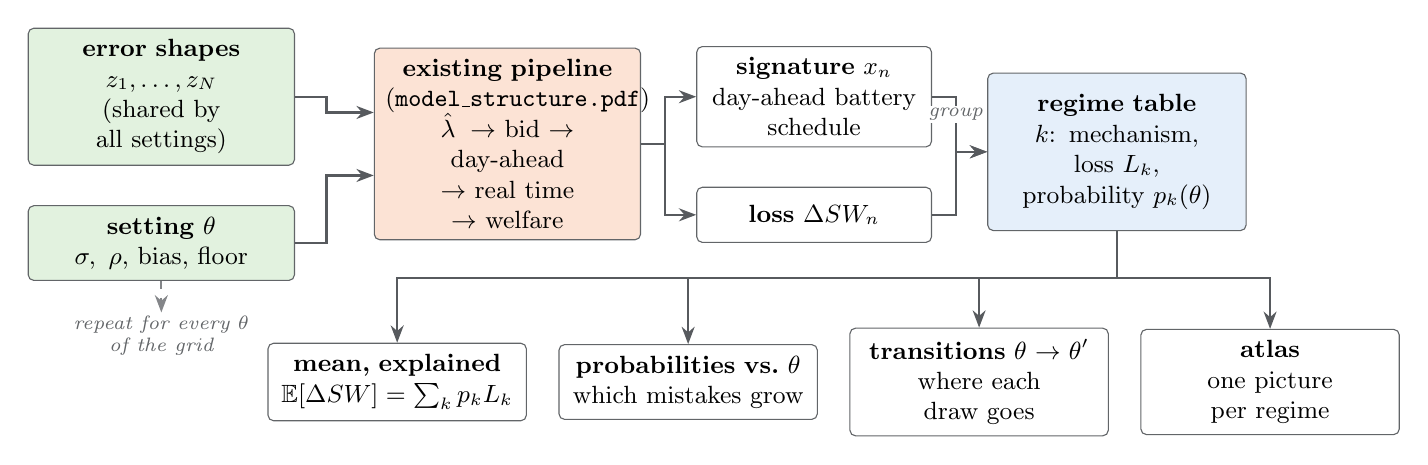
\begin{tikzpicture}[node distance=6mm and 7mm]
  \node[datbox, text width=31mm] (bank) {\textbf{error shapes}\\$z_1,\dots,z_N$\\(shared by all settings)};
  \node[datbox, below=5mm of bank, text width=31mm] (theta) {\textbf{setting} $\theta$\\$\sigma,\ \rho,\ $bias, floor};
  \node[lpbox, right=10mm of bank, yshift=-6mm, text width=31mm, minimum height=20mm] (pipe)
       {\textbf{existing pipeline}\\(\code{model\_structure.pdf})\\$\lamhat\to$ bid $\to$ day-ahead\\$\to$ real time $\to$ welfare};
  \node[box, right=of pipe, text width=27mm, yshift=6mm] (sig) {\textbf{signature} $x_n$\\day-ahead battery\\schedule};
  \node[box, right=of pipe, text width=27mm, yshift=-9mm] (loss) {\textbf{loss} $\Delta SW_n$};
  \node[box, fill=accent!12, right=of sig, yshift=-7mm, text width=30mm, minimum height=20mm] (tab)
       {\textbf{regime table}\\$k$: mechanism,\\loss $L_k$,\\probability $p_k(\theta)$};
  \draw[arr] (bank.east) -- ++(4mm,0) |- ([yshift=4mm]pipe.west);
  \draw[arr] (theta.east) -- ++(4mm,0) |- ([yshift=-4mm]pipe.west);
  \draw[arr] (pipe.east) -- ++(3mm,0) |- (sig.west);
  \draw[arr] (pipe.east) -- ++(3mm,0) |- (loss.west);
  \draw[arr] (sig.east) -- ++(3mm,0) |- node[lab, pos=0.25, above]{group} (tab.west);
  \draw[arr] (loss.east) -- ++(3mm,0) |- (tab.west);
  % outputs
  \node[box, fill=white, below=13mm of pipe, xshift=-14mm, text width=30mm] (o1) {\textbf{mean, explained}\\$\E[\Delta SW]=\sum_k p_k L_k$};
  \node[box, fill=white, right=4mm of o1, text width=30mm] (o2) {\textbf{probabilities vs.\ $\theta$}\\which mistakes grow};
  \node[box, fill=white, right=4mm of o2, text width=30mm] (o3) {\textbf{transitions} $\theta\to\theta'$\\where each draw goes};
  \node[box, fill=white, right=4mm of o3, text width=30mm] (o4) {\textbf{atlas}\\one picture per regime};
  \draw[arr] (tab.south) -- ++(0,-6mm) -| (o4.north);
  \draw[arr] (tab.south) -- ++(0,-6mm) -| (o3.north);
  \draw[arr] (tab.south) -- ++(0,-6mm) -| (o2.north);
  \draw[arr] (tab.south) -- ++(0,-6mm) -| (o1.north);
  \draw[darr] (theta.south) -- ++(0,-4mm) node[lab, below, align=center]{repeat for every $\theta$\\of the grid};
\end{tikzpicture}
\end{center}

Nothing in the model changes: the regimes are a way of \emph{reading} the experiment outputs. Two ingredients
are new: (i) the same error shapes $z_n$ are reused for every setting (common random numbers), and (ii) every
draw records its signature next to its loss.

\textbf{What it adds to the thesis.}
\begin{itemize}
  \item \textbf{Explains the mean.} A rise of the mean loss with $\sigma$ becomes ``regime $k$ becomes more
    likely'': a mechanism, not only a number.
  \item \textbf{Shows the tail.} A rare, expensive regime is visible with its probability, instead of being
    averaged away.
  \item \textbf{Answers ``how often does this happen''.} Each regime carries a probability under the error
    model; with calibrated or empirical errors (stage~3) that becomes a frequency in a real market.
  \item \textbf{Cleaner comparisons.} With common random numbers, the difference between two settings is the
    net flow of draws between regimes, with far less noise than two independent samples.
\end{itemize}

% =====================================================================
\section{Why cluster by outcome, not by error shape}
% =====================================================================

The error shape $z\in\mathbb R^T$ is the natural thing to cluster, but it is the wrong one. The market
outcome is a \emph{piecewise-constant} function of $z$: $z$-space is cut into cells by threshold hyperplanes,
and inside a cell nothing in the market changes. Two shapes that are close but on opposite sides of a
threshold give different outcomes; two that are far apart in the same cell give the same one. Clustering
$z$ (e.g.\ $k$-means) would mix cells; clustering the outcome recovers them exactly.

\begin{center}
\begin{minipage}[c]{0.42\textwidth}
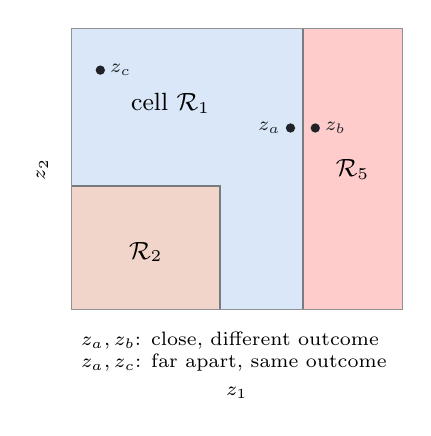
\begin{tikzpicture}[scale=1.05]
  \fill[accent!18] (0,0) rectangle (4,3.4);
  \fill[warn!22] (0,0) -- (1.8,0) -- (1.8,1.5) -- (0,1.5) -- cycle;
  \fill[red!20] (2.8,0) rectangle (4,3.4);
  \draw[ink!60, thick] (1.8,0) -- (1.8,1.5) -- (0,1.5);
  \draw[ink!60, thick] (2.8,0) -- (2.8,3.4);
  \draw[ink!50] (0,0) rectangle (4,3.4);
  \node[font=\small] at (1.2,2.5) {cell $\R_1$};
  \node[font=\small] at (0.9,0.7) {$\R_2$};
  \node[font=\small] at (3.4,1.7) {$\R_5$};
  \fill[ink] (2.65,2.2) circle (1.6pt) node[left, font=\scriptsize]{$z_a$};
  \fill[ink] (2.95,2.2) circle (1.6pt) node[right, font=\scriptsize]{$z_b$};
  \fill[ink] (0.35,2.9) circle (1.6pt) node[right, font=\scriptsize]{$z_c$};
  \node[font=\scriptsize, align=left, anchor=north west] at (0,-0.15)
    {$z_a,z_b$: close, different outcome\\$z_a,z_c$: far apart, same outcome};
  \node[font=\scriptsize, rotate=90] at (-0.35,1.7) {$z_2$};
  \node[font=\scriptsize] at (2,-1.0) {$z_1$};
\end{tikzpicture}
\end{minipage}\hfill
\begin{minipage}[c]{0.55\textwidth}
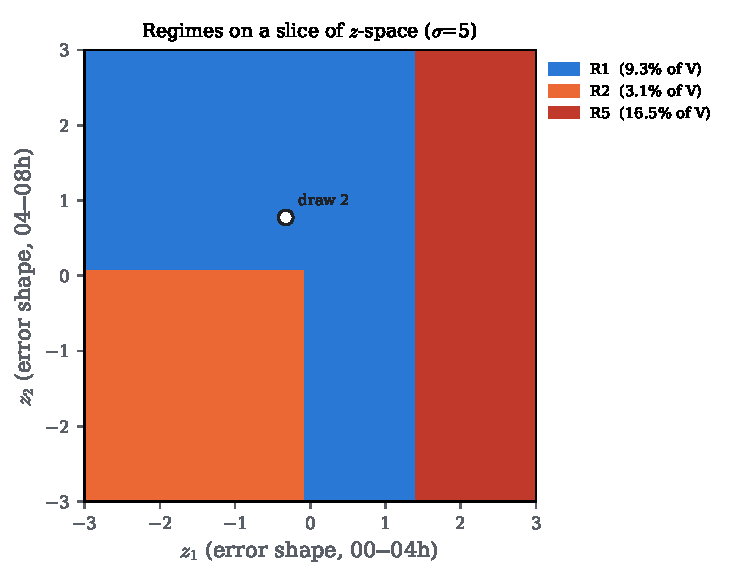
\includegraphics[width=\textwidth]{figures/reg_map.pdf}
\end{minipage}
\end{center}
{\small Left: the principle. Right: the real partition of the test system on a 2-D slice of $z$-space
($z_1, z_2$ vary, the other four intervals fixed at the values of a typical draw, $\sigma=5$\,\$/MWh). The
boundaries are straight lines, because a threshold on the forecast $\lamhat_t = \lamstar_t+\sigma z_t$ is a
threshold on $z_t$. Crossing $z_1\approx1.4$ (a forecast about 7\,\$/MWh too high at 00--04h) moves the draw
from $\R_1$ (9.3\% of $V$) to $\R_5$ (16.5\%).}

% =====================================================================
\section{The mathematics}
% =====================================================================

\subsection{The chain, at a glance}
\begin{center}
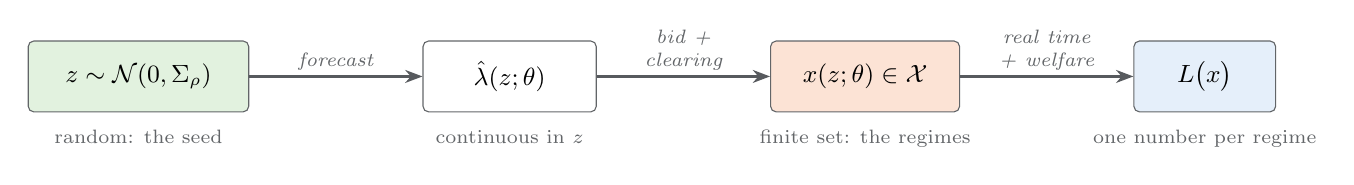
\begin{tikzpicture}[node distance=5mm and 22mm]
  \node[datbox, minimum width=28mm, minimum height=9mm] (z) {$z\sim\mathcal N(0,\Sigma_\rho)$};
  \node[box, right=of z, minimum width=22mm, minimum height=9mm] (l) {$\lamhat(z;\theta)$};
  \node[lpbox, right=of l, minimum width=24mm, minimum height=9mm] (x) {$x(z;\theta)\in\mathcal X$};
  \node[box, fill=accent!12, right=of x, minimum width=18mm, minimum height=9mm] (L) {$L\big(x\big)$};
  \draw[arr] (z) -- node[lab, above=1pt, fill=none]{forecast} (l);
  \draw[arr] (l) -- node[lab, above=1pt, fill=none, align=center]{bid +\\clearing} (x);
  \draw[arr] (x) -- node[lab, above=1pt, fill=none, align=center]{real time\\+ welfare} (L);
  \node[font=\scriptsize, below=1mm of z, text=ink!70] {random: the seed};
  \node[font=\scriptsize, below=1mm of l, text=ink!70] {continuous in $z$};
  \node[font=\scriptsize, below=1mm of x, text=ink!70] {finite set: the regimes};
  \node[font=\scriptsize, below=1mm of L, text=ink!70] {one number per regime};
\end{tikzpicture}
\end{center}

\subsection{Draws and settings}
One battery, $T$ intervals. A draw is an error shape $z\in\mathbb R^T$, Gaussian with the AR(1) covariance
\[
z\sim\mathcal N(0,\Sigma_\rho),\qquad (\Sigma_\rho)_{ts}=\rho^{|t-s|},
\]
(with one battery the common/specific split $\omega$ has no effect). A setting $\theta=(\sigma,\rho,b,
\underline\lambda,\text{rule},\psi)$ turns it into a forecast (\code{model\_structure.pdf}, \S5):
\[
\lamhat(z;\theta)=\max\big(\underline\lambda,\ \lamstar+b\,\bar\lambda+\sigma z\big).
\]
$\rho$ enters through $\Sigma_\rho$; in the code the same random numbers produce $z$ for every $\rho$, so
common random numbers also hold across $\rho$.

\subsection{The outcome map and the regimes}
Let $x(z;\theta)$ be the battery's day-ahead schedule $(p^{da}_t,g^{da}_t)_{t=1}^T$ produced by bid
construction and clearing (M3--M5). Every LP in that chain returns a vertex solution, so $x$ takes values in
a \emph{finite} set $\mathcal X=\{x_1,x_2,\dots\}$, and is constant between thresholds. A \textbf{regime} is
the set of error shapes that produce the same schedule:
\[
\R_k(\theta)=\{z\in\mathbb R^T:\ x(z;\theta)=x_k\},\qquad
\textstyle\bigcup_k\R_k(\theta)=\mathbb R^T,\quad \R_k\cap\R_l=\emptyset\ (k\ne l).
\]
Its probability under the error model is $p_k(\theta)=\Pr\big(z\in\R_k(\theta)\big)$, with $\sum_kp_k=1$.

\subsection{The loss is a regime constant, so the mean decomposes exactly}
Given the day-ahead schedule, everything after it is deterministic and uses only the true system: the
real-time repair (M6) takes $(p^{da},g^{da})$, the redispatch (M7) takes the generators' day-ahead dispatch,
which the hourly clearing fixes from the net demand $D_t+p^{da}_t-g^{da}_t$, and welfare is evaluated at the
true parameters. Hence the loss depends on $z$ only through the regime:
\[
\Delta SW(z;\theta)=L\big(x(z;\theta);\psi\big)=L_k\quad\text{for }z\in\R_k(\theta),
\]
and the moments of the loss are exact finite sums:
\[
\boxed{\ \E[\Delta SW\mid\theta]=\sum_k p_k(\theta)\,L_k,\qquad
\operatorname{Var}[\Delta SW\mid\theta]=\sum_kp_k(\theta)\big(L_k-\E[\Delta SW\mid\theta]\big)^2\ }
\]
The argument needs the generators' day-ahead dispatch to be unique given the net demand; with tied generator
costs it could depend on the bids too. The prototype checks the claim directly: across 2\,400 draws the
largest loss difference within a regime is \textbf{0.0} (\S\ref{sec:proto}).

\subsection{Estimation}
With $N$ draws $z_1,\dots,z_N$ and $n_k=\#\{n: x(z_n;\theta)=x_k\}$:
\[
\hat p_k=\frac{n_k}{N},\qquad \operatorname{se}(\hat p_k)=\sqrt{\frac{\hat p_k(1-\hat p_k)}{N}},\qquad
\hat\mu=\sum_k\hat p_kL_k=\frac1N\sum_{n}\Delta SW(z_n;\theta).
\]
The decomposed mean is \emph{identical} to the Monte Carlo mean (not an approximation); the regime table only
re-arranges it. Regimes never seen in the sample have $\hat p_k=0$; the chance of missing a regime of
probability $p$ is $(1-p)^N$ (0.7\% for $p=1\%$ at $N=500$).

\subsection{Comparing two settings: transitions under common random numbers}
Use the \emph{same} $z_n$ under $\theta$ and $\theta'$. The transition matrix
\[
P_{kl}(\theta\to\theta')=\frac1N\,\#\{n:\ x(z_n;\theta)=x_k,\ x(z_n;\theta')=x_l\}
\]
has row sums $\hat p_k(\theta)$ and column sums $\hat p_l(\theta')$, and splits the change in mean loss into
flows between regimes:
\[
\hat\mu(\theta')-\hat\mu(\theta)=\sum_{k,l}P_{kl}\,\big(L_l-L_k\big).
\]
Draws that stay in their regime ($k=l$) contribute nothing, which is why common random numbers make the
comparison so much less noisy: only the draws that \emph{cross a threshold} carry the difference.

\subsection{Naming the regimes: mechanism features}
A regime key is a long vector of MW; for reading it is described by a few features of its outcome:
\begin{center}\footnotesize
\begin{tabular}{@{}lll@{}}
\toprule
Feature & Definition & Reads as \\
\midrule
pattern & per interval: C (charges), D (discharges), -- (idle), day-ahead & what the battery sold \\
$E^{\text{free}}$ & $\Delta T\sum_{t:\lamstar_t=0}p^{da}_t$ & did it buy the free energy? \\
infeasible intervals & $\#\{t: s^{da}_t\notin[\underline s,\bar s]\}$ & how wrong the day-ahead plan is \\
undeliverable & $\Delta T\sum_t|p_t-p^{da}_t|+|g_t-g^{da}_t|$ & how much real time must correct \\
shed & $\Delta T\sum_t sh_t$ & did it cause load shedding? \\
thermal at cheap hours & $\Delta T\sum_{t:\,p^{da}_t>0}q^{rt}_{\text{thermal},t}$ & did it charge from expensive supply? \\
\bottomrule
\end{tabular}
\end{center}
A short rule-based label is generated from them (``missed morning sale'', ``charges from thermal at
00--04h'', \dots); the label is for reading only, the regime is still defined by the exact schedule.

\subsection{Larger systems: when the loss is not constant within a signature}
With 24 intervals, ramps, several batteries or a network, (i) exact schedules may almost never repeat, and
(ii) the real-time outcome can depend on more than the day-ahead battery schedule. Then:
\begin{itemize}
  \item use a \textbf{coarse signature} (the feature vector above, rounded) or cluster the standardised
    feature vectors with $k$-medoids, choosing $K$ by silhouette;
  \item the decomposition still holds with \emph{conditional} means,
    $\E[\Delta SW]=\sum_kp_k\,\E[\Delta SW\mid k]$, and the within-regime spread
    $\operatorname{Var}[\Delta SW\mid k]$ is reported next to each regime as a quality measure of the clustering.
\end{itemize}

\subsection{From model probabilities to ``how often in reality''}
$p_k(\theta)$ is a probability \emph{under the error model}. Two routes make it a real-market frequency
(stage~3):
\begin{enumerate}
  \item \textbf{Calibrate, then sample:} estimate $\sigma$, $\rho$, bias from a backtest of real forecasts
    and read $p_k$ at the calibrated $\theta$.
  \item \textbf{Empirical shapes:} replace the Gaussian bank by real forecast-error days $z^{\text{emp}}_n$
    (\code{forecasts.bootstrap\_days}); then $\hat p_k$ is directly the share of real days in regime $k$.
    Existing Gaussian draws can also be re-weighted to an empirical density $f$ with importance weights:
    \[
    w_n=\frac{f(z_n)}{\varphi_{\Sigma_\rho}(z_n)},\qquad
    \hat p_k=\frac{\sum_n w_n\,\mathbf 1[z_n\in\R_k]}{\sum_nw_n}.
    \]
\end{enumerate}

% =====================================================================
\section{First look: the prototype}
\label{sec:proto}
% =====================================================================

\code{docs/prototypes/regimes\_prototype.py}: test system \code{day\_case}, \code{B\_fcst}, prelimit rule,
$\psi=10$, price floor 0, $\rho=0$; $N=400$ error shapes (seeds $0,\dots,399$) reused for every
$\sigma\in\{0.5,1,2,5,10,20\}$\,\$/MWh. These are exploratory numbers that show the method works; the real
runs follow \S\ref{sec:code}.

\textbf{Checks.} Loss constant within every regime (largest spread 0.0); $\sum_k\hat p_kL_k$ equals the
Monte Carlo mean at every $\sigma$ (e.g.\ 6.8132 = 6.8132 at $\sigma=5$); 31 distinct regimes in total,
14--28 per $\sigma$; the 7 most frequent cover 87\% of draws at $\sigma=1$ and 70\% at $\sigma=20$; the
transition flows between $\sigma=1$ and $\sigma=5$ add up exactly to the change in mean loss ($+0.558$).

\begin{center}\footnotesize
\begin{tabular}{@{}clrccccl@{}}
\toprule
 & pattern & loss & \multicolumn{3}{c}{probability at $\sigma=$} & undeliv. & mechanism \\
\cmidrule(lr){4-6}
 & (00h $\to$ 24h) & (\% of $V$) & 1 & 5 & 20 & (MWh) & \\
\midrule
$\R_1$ & \code{C-CCDD} & 9.31 & 0.405 & 0.362 & 0.185 & 1\,371 & keeps the morning charge, no 04--08h sale \\
$\R_2$ & \code{CDCCDD} & 3.09 & 0.130 & 0.128 & 0.122 & 1\,051 & benchmark-like cycle, oversells the evening \\
$\R_3$ & \code{C--CDD} & 2.83 & 0.133 & 0.098 & 0.060 & 580 & charges in only one free interval \\
$\R_4$ & \code{C-CCDD} & 8.70 & 0.087 & 0.077 & 0.045 & 1\,071 & as $\R_1$, but sells less at 16--20h \\
$\R_5$ & \code{C-CCDD} & 16.46 & 0 & 0.052 & 0.223 & 1\,731 & buys 200\,MW from thermal at 00--04h \\
$\R_6$ & \code{C-CCD-} & 4.47 & 0.068 & 0.062 & 0.035 & 1\,071 & holds energy to the end of the day \\
$\R_7$ & \code{CD-CDD} & 2.36 & 0.045 & 0.040 & 0.028 & 420 & sells in the morning, one free interval \\
\midrule
 & mean $\sum_kp_kL_k$ & & 6.26 & 6.81 & 8.86 & & \\
\bottomrule
\end{tabular}
\end{center}
{\small $\R_1$, $\R_4$ and $\R_5$ share the on/off pattern but differ in MW; the features (undeliverable
energy, thermal use) tell them apart. Benchmark schedule for reference: charge 100/0/200/22/0/0\,MW,
discharge 0/90/0/0/175/25\,MW.}

\begin{center}
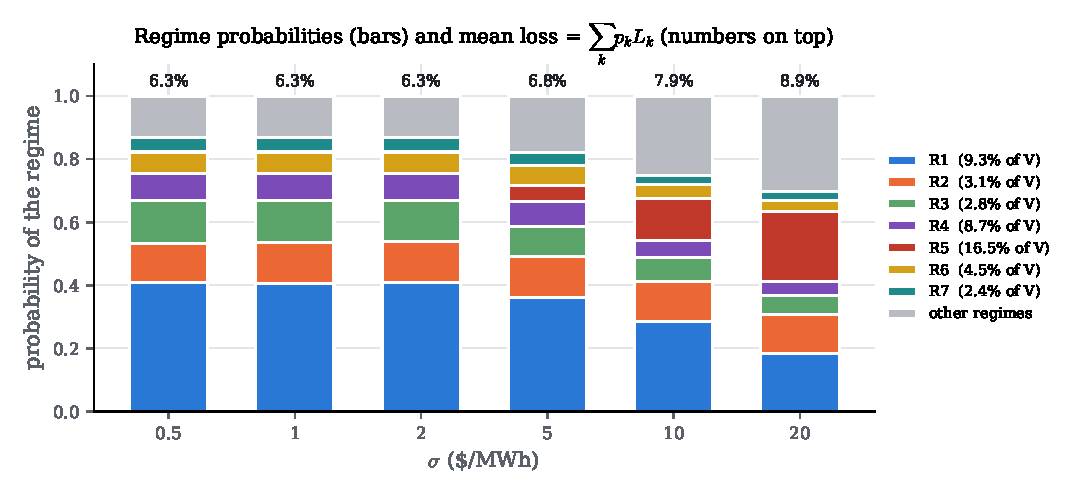
\includegraphics[width=0.86\textwidth]{figures/reg_probabilities.pdf}
\end{center}
{\small \textbf{How $\sigma$ raises the mean loss.} Up to $\sigma=2$ the regime mix is almost unchanged
(mean 6.3\%). From $\sigma=5$ on, $\R_1$ (9.3\%) loses draws and $\R_5$ (16.5\%) gains them: at
$\sigma=20$, $\R_5$ is the most likely single regime. The rise of the mean (6.3\% $\to$ 8.9\%) is mainly this
one shift, plus a growing tail of rare regimes (``other'').}

\begin{center}
\begin{minipage}[c]{0.5\textwidth}
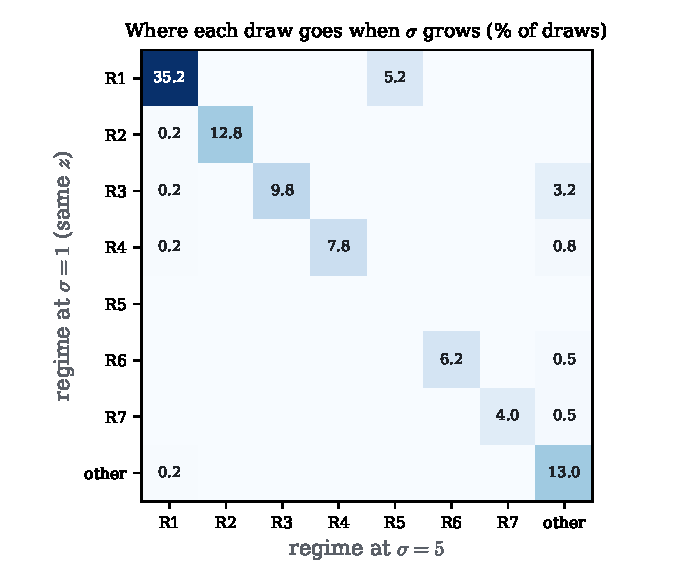
\includegraphics[width=\textwidth]{figures/reg_transitions.pdf}
\end{minipage}\hfill
\begin{minipage}[c]{0.46\textwidth}\small
\textbf{Where each draw goes} (same 400 error shapes at $\sigma=1$ and $\sigma=5$). 88\% of draws stay in
their regime (diagonal) and contribute nothing. The mean rises by $+0.558$ points of $V$, and the flows add
up to exactly that: $\R_1\to\R_5$ (21 draws, $+7.2$ points each) contributes $+0.376$, two thirds of the
change; $\R_4\to\R_{11}$ ($+0.054$), $\R_3\to\R_{12},\R_{18}$ ($+0.054$) and $\R_6\to\R_{15}$
($+0.033$) most of the rest. One flow lowers the loss ($\R_8\to\R_{19}$, $-0.010$).
\end{minipage}
\end{center}

% =====================================================================
\section{Code topology: how it plugs into the existing code}
\label{sec:code}
% =====================================================================

The regime analysis is a \emph{reader} of the existing pipeline: it reuses bid construction, clearing,
real-time repair and welfare unchanged (\code{runner.evaluate\_blocks}) and adds one module, one script,
one notebook and one test file. Two existing modules get small, behaviour-preserving changes.

\begin{center}
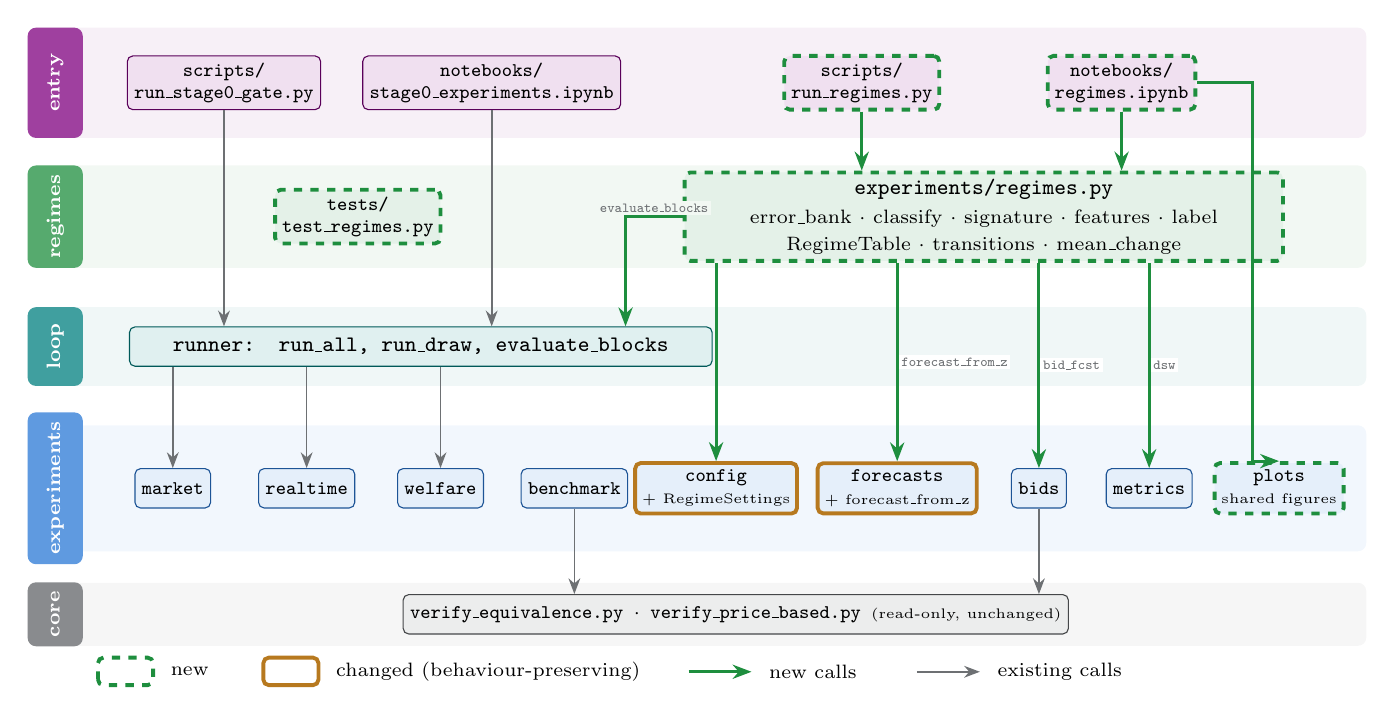
\begin{tikzpicture}[
  lane/.style={draw=none, rounded corners=3pt, minimum width=17cm, anchor=west},
  tab/.style={rounded corners=3pt, minimum width=7mm, anchor=west, text=white, font=\scriptsize\bfseries},
  chip/.style={draw=#1!70!black, fill=#1!12, rounded corners=2pt, font=\ttfamily\scriptsize, inner sep=2.5pt,
               minimum height=5mm, align=center},
  newb/.style={line width=1.4pt, draw=newc, dashed},
  chgb/.style={line width=1.4pt, draw=chg},
  imp/.style={-{Stealth[length=2mm]}, semithick, ink!65},
  newarr/.style={-{Stealth[length=2.4mm]}, line width=1.1pt, newc},
  ilab/.style={font=\tiny\ttfamily, text=ink!65, fill=white, inner sep=1pt},
]
\colorlet{cE}{violet}\colorlet{cO}{teal}\colorlet{cX}{accent}\colorlet{cC}{ink!70}\colorlet{cR}{newc}
\foreach \y/\h/\c/\t in {-0.8/1.4/cE/entry, -2.5/1.3/cR/regimes, -4.15/1.0/cO/loop, -5.95/1.6/cX/experiments, -7.55/0.8/cC/core} {
  \node[lane, fill=\c!6, minimum height=\h cm] at (0,\y) {};
  \node[tab, fill=\c!75, minimum height=\h cm] at (0,\y) {\rotatebox{90}{\t}};
}
% entry: existing on the left, new on the right
\node[chip=cE] (gate) at (2.5,-0.8) {scripts/\\run\_stage0\_gate.py};
\node[chip=cE] (snb) at (5.9,-0.8) {notebooks/\\stage0\_experiments.ipynb};
\node[chip=cE, newb] (rscr) at (10.6,-0.8) {scripts/\\run\_regimes.py};
\node[chip=cE, newb] (rnb) at (13.9,-0.8) {notebooks/\\regimes.ipynb};
% regimes layer (new), right half
\node[chip=cR, newb, font=\ttfamily\footnotesize, minimum width=7.6cm, minimum height=10mm] (reg) at (12.15,-2.5)
  {experiments/regimes.py\\[1pt]{\rmfamily\scriptsize error\_bank $\cdot$ classify $\cdot$ signature $\cdot$ features $\cdot$ label}\\
   {\rmfamily\scriptsize RegimeTable $\cdot$ transitions $\cdot$ mean\_change}};
\node[chip=cR, newb] (rtest) at (4.2,-2.5) {tests/\\test\_regimes.py};
% loop (existing), left half
\node[chip=cO, minimum width=7.4cm, font=\ttfamily\footnotesize] (run) at (5.0,-4.15)
  {runner: run\_all, run\_draw, evaluate\_blocks};
% experiments: under the runner what it drives; under regimes what regimes calls
\node[chip=cX] (mk) at (1.85,-5.95) {market};
\node[chip=cX] (rtm) at (3.55,-5.95) {realtime};
\node[chip=cX] (wf) at (5.25,-5.95) {welfare};
\node[chip=cX] (bn) at (6.95,-5.95) {benchmark};
\node[chip=cX, chgb] (cfg) at (8.75,-5.95) {config\\{\rmfamily\tiny + RegimeSettings}};
\node[chip=cX, chgb] (fc) at (11.05,-5.95) {forecasts\\{\rmfamily\tiny + forecast\_from\_z}};
\node[chip=cX] (bid) at (12.85,-5.95) {bids};
\node[chip=cX] (me) at (14.25,-5.95) {metrics};
\node[chip=cX, newb] (pl) at (15.9,-5.95) {plots\\{\rmfamily\tiny shared figures}};
% core
\node[chip=cC] (core) at (9.0,-7.55) {verify\_equivalence.py $\cdot$ verify\_price\_based.py {\rmfamily\tiny (read-only, unchanged)}};
% existing calls
\draw[imp] (gate.south) -- (gate.south |- run.north);
\draw[imp] (snb.south) -- (snb.south |- run.north);
\foreach \m in {mk, rtm, wf} \draw[imp] (run.south -| \m.north) -- (\m.north);
\draw[imp] (bid.south) -- (bid.south |- core.north);
\draw[imp] (bn.south) -- (bn.south |- core.north);
% new calls, all downward
\draw[newarr] (rscr.south) -- (rscr.south |- reg.north);
\draw[newarr] (rnb.south) -- (rnb.south |- reg.north);
\draw[newarr] (reg.south -| cfg.north) -- (cfg.north);
\draw[newarr] (reg.south -| fc.north) -- (fc.north) node[ilab, pos=0.5, right]{forecast\_from\_z};
\draw[newarr] (reg.south -| bid.north) -- (bid.north) node[ilab, pos=0.5, right]{bid\_fcst};
\draw[newarr] (reg.south -| me.north) -- (me.north) node[ilab, pos=0.5, right]{dsw};
\draw[newarr] (reg.west) -- (7.6,-2.5) node[ilab, pos=0.5, above, fill=cR!6]{evaluate\_blocks} -- (7.6,-4.15 |- run.north);
\draw[newarr] (rnb.east) -- ++(0.7,0) |- (pl.north);
% legend
\draw[newb, rounded corners=2pt] (0.9,-8.45) rectangle ++(0.7,0.35); \node[font=\scriptsize, anchor=west] at (1.7,-8.28) {new};
\draw[chgb, rounded corners=2pt] (3.0,-8.45) rectangle ++(0.7,0.35); \node[font=\scriptsize, anchor=west] at (3.8,-8.28) {changed (behaviour-preserving)};
\draw[newarr] (8.4,-8.28) -- ++(0.8,0); \node[font=\scriptsize, anchor=west] at (9.3,-8.28) {new calls};
\draw[imp] (11.3,-8.28) -- ++(0.8,0); \node[font=\scriptsize, anchor=west] at (12.2,-8.28) {existing calls};
\end{tikzpicture}
\end{center}

{\small The new \textbf{regimes} layer sits between the entry points and the experiment modules. It calls
\code{forecasts} (shapes $\to$ forecasts), \code{bids} (the \code{B\_fcst} bid), \code{runner.evaluate\_blocks}
(clearing, real time, welfare: unchanged) and \code{metrics.dsw}. \code{plots} collects the figure helpers that
today live inside the stage-0 notebook (it is already foreseen in \code{experiments.md} \S3), so both notebooks
share them.}

\subsection{What is new and what changes}
\begin{center}\small
\begin{tabularx}{\textwidth}{@{}l>{\raggedright\arraybackslash}X>{\raggedright\arraybackslash}p{4.4cm}@{}}
\toprule
File & Role & Main objects \\
\midrule
\multicolumn{3}{@{}l}{\textcolor{newc}{\textbf{new}}}\\
\code{experiments/regimes.py} & Error-shape bank, classification of draws into regimes, features and labels, regime
tables, transitions, decomposition of mean changes. & \code{error\_bank}, \code{classify}, \code{signature},
\code{features}, \code{label}, \code{RegimeTable}, \code{transitions}, \code{mean\_change} \\
\code{experiments/plots.py} & Figure helpers shared by the notebooks (energy balance, SOC axes, bid bands, the
eight-panel draw, regime charts). & \code{energy\_balance}, \code{draw\_panels}, \code{regime\_bars},
\code{transition\_matrix} \\
\code{scripts/run\_regimes.py} & Runs a grid of settings on one bank, writes results, prints the regime table. &
\code{main} \\
\code{notebooks/regimes.ipynb} & The regime atlas: table, probability chart, transitions, one picture per
regime, a regime explorer. & -- \\
\code{tests/test\_regimes.py} & Acceptance tests (\S\ref{sec:tests}). & -- \\
\code{results/regimes/} & One CSV row per (setting, draw) with regime id and features; \code{regimes.json} with
the regime dictionary; \code{meta.json}. & git-ignored \\
\midrule
\multicolumn{3}{@{}l}{\textcolor{chg}{\textbf{changed, behaviour-preserving}}}\\
\code{experiments/forecasts.py} & Split \code{forecast\_prices} into ``draw the shapes'' and ``apply $\theta$ to
a shape''; \code{forecast\_prices} calls both and returns identical numbers. & \code{error\_shapes},
\code{forecast\_from\_z} \\
\code{experiments/config.py} & \code{RegimeSettings}. (Stable per-draw seeds from (\code{base\_seed}, \code{draw})
only, i.e.\ common random numbers and reproducible draws: \textbf{done} on 28 Oct 2026, \code{RunSettings.seed}.) & \code{RegimeSettings} \\
\bottomrule
\end{tabularx}
\end{center}

\subsection{Data flow of one regime run}
\begin{center}
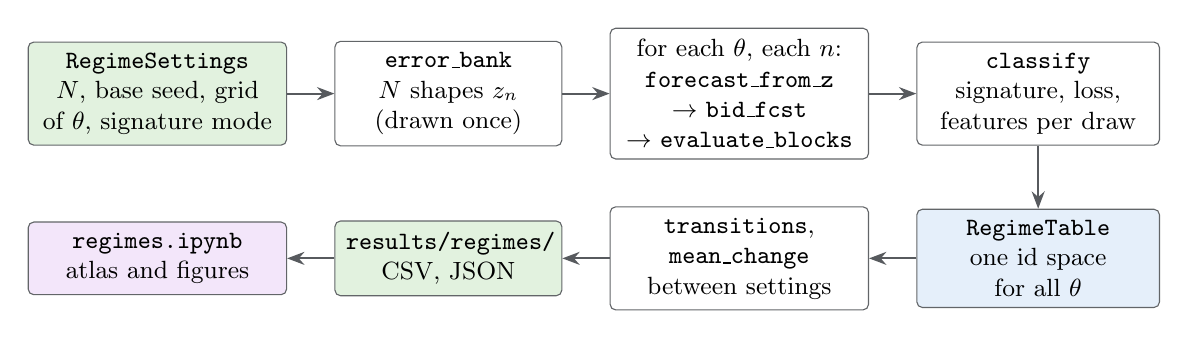
\begin{tikzpicture}[node distance=5mm and 6mm]
  \node[datbox, text width=30mm] (rs) {\code{RegimeSettings}\\$N$, base seed, grid of $\theta$, signature mode};
  \node[box, fill=white, right=of rs, text width=26mm] (bank) {\code{error\_bank}\\$N$ shapes $z_n$\\(drawn once)};
  \node[box, fill=white, right=of bank, text width=30mm] (loop) {for each $\theta$, each $n$:\\\code{forecast\_from\_z}\\$\to$ \code{bid\_fcst}\\$\to$ \code{evaluate\_blocks}};
  \node[box, fill=white, right=of loop, text width=28mm] (cls) {\code{classify}\\signature, loss,\\features per draw};
  \node[box, fill=accent!12, below=8mm of cls, text width=28mm] (tab) {\code{RegimeTable}\\one id space for all $\theta$};
  \node[box, fill=white, left=of tab, text width=30mm] (tr) {\code{transitions},\\\code{mean\_change}\\between settings};
  \node[datbox, left=of tr, text width=26mm] (out) {\code{results/regimes/}\\CSV, JSON};
  \node[drvbox, left=of out, text width=30mm, font=\small] (nb) {\code{regimes.ipynb}\\atlas and figures};
  \draw[arr] (rs) -- (bank); \draw[arr] (bank) -- (loop); \draw[arr] (loop) -- (cls); \draw[arr] (cls) -- (tab);
  \draw[arr] (tab) -- (tr); \draw[arr] (tr) -- (out); \draw[arr] (out) -- (nb);
\end{tikzpicture}
\end{center}
{\small Cost: one draw takes about 0.03\,s, so $N=500$ draws per setting is 15\,s, and the 324-setting stage-1
grid about 80 minutes; the regime layer itself only groups numbers (negligible).}

\subsection{Interfaces (sketch)}
{\footnotesize
\begin{verbatim}
# experiments/forecasts.py  (split; forecast_prices returns the same numbers as today)
def error_shapes(T, error, n_ess, rng) -> np.ndarray        # z, shape (n_ess, T)
def forecast_from_z(lam_star, z, error) -> np.ndarray       # max(floor, lam* + bias + sigma*z)

# experiments/regimes.py
def error_bank(n, T, rho, base_seed) -> np.ndarray          # (n, T), shared by every setting
def signature(outcome, mode="day_ahead") -> tuple           # the regime key
def features(case, outcome) -> dict                         # free energy, infeasible, shed, ...
def label(features) -> str                                  # "missed morning sale", ...
def classify(case, bench, bank, error, bid_rule, rt) -> pd.DataFrame   # one row per draw

@dataclass
class RegimeTable:                                          # one id space for all settings
    regimes: pd.DataFrame       # id, key, pattern, label, loss, features
    probs: pd.DataFrame         # (setting, id) -> p, se
    def mean_loss(self, setting) -> float                   # sum_k p_k L_k

def transitions(draws_a, draws_b) -> pd.DataFrame           # P_kl on the same bank
def mean_change(draws_a, draws_b, table) -> pd.DataFrame    # flows k -> l and L_l - L_k
\end{verbatim}
}

\subsection{Acceptance tests}
\label{sec:tests}
\begin{center}\small
\begin{tabularx}{\textwidth}{@{}l>{\raggedright\arraybackslash}X@{}}
\toprule
Test & Passes when \\
\midrule
same numbers after the split & \code{forecast\_from\_z(error\_shapes(...))} equals \code{forecast\_prices} for the same seed, bit for bit \\
probabilities & $\sum_k\hat p_k=1$ for every setting \\
exact decomposition & $\sum_k\hat p_kL_k$ equals the Monte Carlo mean of the loss to $10^{-9}$ \\
regime constant & in \code{day\_case}, the loss spread within every regime is below $10^{-9}$ (else the coarse-signature mode is required) \\
zero error & at $\sigma=0$ there is one regime, with the \code{B\_star\_p} loss (6.32\% of $V$) \\
transitions & row sums of $P$ equal $\hat p(\theta)$, column sums equal $\hat p(\theta')$; $\sum_{k,l}P_{kl}(L_l-L_k)=\hat\mu(\theta')-\hat\mu(\theta)$ \\
reproducible & the same \code{base\_seed} gives the same bank and the same table in a new Python session \\
\bottomrule
\end{tabularx}
\end{center}

\subsection{Work plan}
\begin{center}
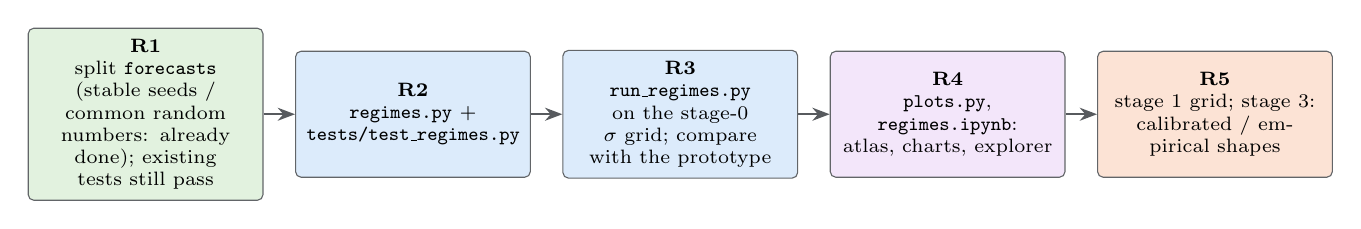
\begin{tikzpicture}[node distance=4mm,
  st/.style={box, text width=27mm, minimum height=16mm, font=\scriptsize}]
  \node[st, fill=dat] (r1) {\textbf{R1}\\split \code{forecasts} (stable seeds / common random numbers: already done); existing tests still pass};
  \node[st, fill=ex, right=of r1] (r2) {\textbf{R2}\\\code{regimes.py} + \code{tests/test\_regimes.py}};
  \node[st, fill=ex, right=of r2] (r3) {\textbf{R3}\\\code{run\_regimes.py} on the stage-0 $\sigma$ grid; compare with the prototype};
  \node[st, fill=drv, right=of r3] (r4) {\textbf{R4}\\\code{plots.py}, \code{regimes.ipynb}: atlas, charts, explorer};
  \node[st, fill=lp, right=of r4] (r5) {\textbf{R5}\\stage~1 grid; stage~3: calibrated / empirical shapes};
  \foreach \a/\b in {r1/r2, r2/r3, r3/r4, r4/r5} \draw[arr] (\a) -- (\b);
\end{tikzpicture}
\end{center}

% =====================================================================
\section{Limitations to state}
% =====================================================================
\begin{itemize}
  \item \textbf{Model probabilities.} Until stage~3, $p_k$ are probabilities under a Gaussian AR(1) error model,
    not observed frequencies.
  \item \textbf{Test-system specific.} The few, crisp regimes come from the ties of this 6-interval case;
    a 24-hour system will need the coarse-signature mode and will show fuzzier clusters.
  \item \textbf{Signature choice.} Grouping by the day-ahead battery schedule is exact here (the loss is a
    regime constant); in larger systems the within-regime spread must be reported.
  \item \textbf{Rare regimes.} With $N$ draws, regimes of probability below about $3/N$ may be missed; the
    ``other'' share and $(1-p)^N$ say how much.
\end{itemize}

{\small\textbf{Reproducing the prototype.} From the \code{Code/} folder, run
\code{docs/prototypes/regimes\_prototype.py} with the \code{DTU\_SYS} Python. It writes the figures
\code{docs/figures/reg\_*.pdf} and the numbers \code{reg\_summary.json} (about 4 minutes).}

\end{document}
